\section{Método}


\begin{frame}

    \frametitle{Conjunto Seguro Sobre Crenças}

    \begin{columns}[c]

        \begin{column}{0.45\textwidth}
            A restrição de chance define uma função $h_b$ sobre a \textbf{crença}:
            \[
                \mathcal{C}_b = \{\boldsymbol{b} \mid h_b(\boldsymbol{b}) \geq 0\}
            \]

            \textbf{Exemplo}: drone em 1D, parede em $x = 2$, exigência $\Pr[x \leq 2] \geq 90\%$:
            \[
                h_b(\boldsymbol{b}) = 2 - \mu - 1{,}28\,\sigma \geq 0
            \]

            {\small Azul: crenças seguras. No ponto vermelho, a probabilidade de colisão é exatamente 10\%.}
        \end{column}

        \begin{column}{0.53\textwidth}
            \centering
            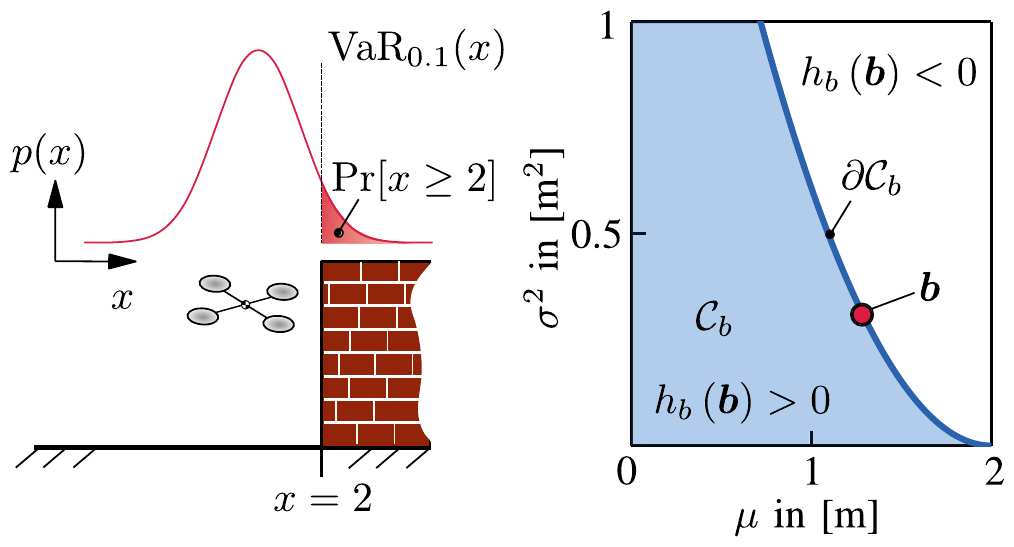
\includegraphics[width=\textwidth]{imagens/fig2_belief_safe_set}

            {\tiny Fonte: \citeonline{vahs2023bcbf}.}
        \end{column}

    \end{columns}

    \vspace{2mm}

    \centering
    \textbf{Ideia}: usar $h_b$ como uma CBF, mas sobre a crença $\boldsymbol{b}$ em vez do estado $\boldsymbol{x}$.

\end{frame}


\begin{frame}

    \frametitle{Como a Crença Evolui: Sistema Híbrido}

    \begin{columns}[c]

        \begin{column}{0.5\textwidth}
            \textbf{Entre medições} (predição do EKF):
            \[
                \dot{\boldsymbol{b}} = \boldsymbol{f}_b(\boldsymbol{b}) + \boldsymbol{g}_b(\boldsymbol{b})\boldsymbol{u}
            \]
            {\small Contínua, determinística e afim em $\boldsymbol{u}$, ou seja, a mesma forma usada nas CBFs. A incerteza \textbf{cresce}.}

            \vspace{3mm}

            \textbf{Na medição} $\boldsymbol{z}_k$ (atualização de Kalman):
            \[
                \boldsymbol{b}^+ = \boldsymbol{\Delta}(\boldsymbol{b}^-)
            \]
            {\small Salto instantâneo e \alert{aleatório}, pois $\boldsymbol{z}_k$ é ruidoso. A incerteza \textbf{cai}.}
        \end{column}

        \begin{column}{0.47\textwidth}
            \centering
            \begin{tikzpicture}[xscale=1.1, yscale=1]
                \draw[->] (0,0) -- (5.2,0) node[below] {\scriptsize $t$};
                \draw[->] (0,0) -- (0,3) node[left] {\scriptsize $\sigma^2$};
                \draw[thick, IFSPPrimario] (0,0.6) .. controls (0.6,1.0) .. (1.2,1.8);
                \draw[thick, IFSPPrimario, dashed] (1.2,1.8) -- (1.2,0.7);
                \draw[thick, IFSPPrimario] (1.2,0.7) .. controls (1.8,1.1) .. (2.4,1.9);
                \draw[thick, IFSPPrimario, dashed] (2.4,1.9) -- (2.4,0.7);
                \draw[thick, IFSPPrimario] (2.4,0.7) .. controls (3.4,1.4) .. (4.4,2.7);
                \draw[thick, IFSPPrimario, dashed] (4.4,2.7) -- (4.4,0.8);
                \foreach \t/\l in {1.2/t_1, 2.4/t_2, 4.4/t_3} {
                    \draw (\t,0.05) -- (\t,-0.05) node[below] {\scriptsize $\l$};
                }
                \node[align=center] at (2.3,2.7) {\scriptsize sem medição\\[-1mm]\scriptsize (ex.: GPS ausente)};
                \draw[->, black!60] (3.1,2.6) -- (3.7,2.0);
            \end{tikzpicture}

            {\scriptsize Variância cresce na predição e cai em cada medição.}
        \end{column}

    \end{columns}

\end{frame}


\begin{frame}

    \frametitle{Belief Control Barrier Functions}

    \begin{block}{Definição (BCBF): a condição de CBF aplicada à crença}
        \[
            \frac{\partial h_b}{\partial \boldsymbol{b}} \big(\boldsymbol{f}_b(\boldsymbol{b}) + \boldsymbol{g}_b(\boldsymbol{b})\boldsymbol{u}\big) \geq -h_b(\boldsymbol{b})
        \]
    \end{block}

    \begin{columns}[c]

        \begin{column}{0.48\textwidth}
            \begin{itemize}
                \item \textbf{Entre medições}: a crença é determinística, logo $\mathcal{C}_b$ é invariante, como na CBF clássica (Teo.~1).
                \item \textbf{Na medição}: um \alert{outlier} pode fazer a crença saltar para fora de $\mathcal{C}_b$.
                \item O artigo \textbf{limita a probabilidade} desse salto (Teo.~2), e a CBF traz a crença de volta.
            \end{itemize}
        \end{column}

        \begin{column}{0.5\textwidth}
            \centering
            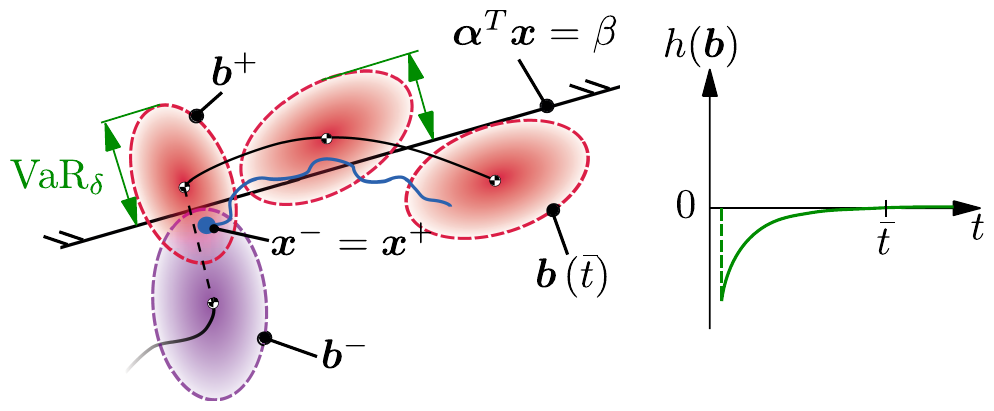
\includegraphics[width=0.95\textwidth]{imagens/fig3_outlier}

            {\tiny Crença $\boldsymbol{b}^-$ segura salta para $\boldsymbol{b}^+$ fora de $\mathcal{C}_b$. Fonte: \citeonline{vahs2023bcbf}.}
        \end{column}

    \end{columns}

\end{frame}


\begin{frame}

    \frametitle{Margem de Segurança e Controle Final}

    \textbf{Evitar o salto para fora}: encolher o conjunto seguro com uma margem $\gamma \geq 0$:
    \[
        \tilde{h}_b(\boldsymbol{b}) = h_b(\boldsymbol{b}) - \gamma
    \]
    {\small Com $\gamma$ escolhido pelo Teorema 3, $\Pr[\boldsymbol{b}^+ \in \mathcal{C}_b] \geq 1 - \varepsilon$ após cada medição.}

    \vspace{2mm}

    \begin{block}{Filtro de segurança (QP), igual ao CBF-QP, mas sobre a crença}
        \[
            \boldsymbol{u}^* = \arg\min_{\boldsymbol{u} \in \mathcal{U}} \; \|\boldsymbol{u} - \boldsymbol{u}_{\text{ref}}\|^2
            \quad \text{s.a.} \quad
            \frac{\partial \tilde{h}_b}{\partial \boldsymbol{b}} \big(\boldsymbol{f}_b(\boldsymbol{b}) + \boldsymbol{g}_b(\boldsymbol{b})\boldsymbol{u}\big) \geq -\tilde{h}_b(\boldsymbol{b})
        \]
    \end{block}

    \begin{itemize}
        \item Otimiza só sobre $\boldsymbol{u}$, não sobre a crença.
        \item Continua sendo um QP $\Rightarrow$ \textbf{tempo real}, até 1\,kHz.
    \end{itemize}

\end{frame}
